\section{Método}
\label{sec:metodo}

\subsection{Protocolo y registro}
\label{sec:met-protocolo}
% PRISMA ítems 24a (registro), 24b (acceso al protocolo), 24c (enmiendas)

% Generado por analysis/src/tablas/tablas.py — no editar a mano.
\begin{table*}[!tbp]
\centering
\caption{Enmiendas al protocolo registrado. Las 3 marcadas como pendientes se actualizarán en el registro OSF antes del envío.}
\label{tab:enmiendas}
\footnotesize
\begin{tabularx}{\textwidth}{@{}l l l p{3.2cm} X l@{}}
\toprule
N.º & Fecha & Fase & Momento respecto de los datos & Cambio & Registro OSF \\
\midrule
A1 & 2026-10-11 & Búsqueda & Antes del cribado (resultados de arXiv y ACL ya conocidos) & La IA determina la elegibilidad del conjunto de referencia; este se usa solo para medir la sensibilidad de la búsqueda. & Actualizada \\
A2 & 2026-10-11 & Búsqueda & Durante la búsqueda & ACM DL se captura guardando las páginas de resultados en HTML; los metadatos se completan por DOI. & Actualizada \\
A3 & 2026-10-11 & Cribado & Antes del cribado & Diseño reducido de verificación humana: una muestra a ciegas (piloto y validación) y revisión de los casos no evidentes. & Actualizada \\
A4 & 2026-10-11 & Recuperación & Tras la recuperación, antes de la extracción & No se contacta a los autores; los informes no recuperados se reportan y se añade una sensibilidad de D4. & Pendiente \\
A5 & 2026-10-12 & Cribado y extracción & Antes de la extracción & Texto completo con revisores Sonnet (y Codex en parte del Nivel 1) y extractos; suplemento de bola de nieve desde Semantic Scholar; extracción doble por IA con verificación por muestreo; variable de nivel del foro. & Pendiente \\
A6 & 2026-10-13 & Síntesis & Durante la síntesis (exploratorio) & Se añaden análisis bibliométricos exploratorios no pre-registrados. & Pendiente \\
\bottomrule
\end{tabularx}
\end{table*}


La revisión sigue las guías de Kitchenham y Charters~\cite{Kitchenham2007Guidelines} y se reporta según PRISMA 2020~\cite{Page2021PRISMA}, con la extensión para búsquedas~\cite{Rethlefsen2021PRISMAS}. El protocolo se redactó según PRISMA-P~\cite{Moher2015PRISMAP} y se registró en OSF antes de las búsquedas oficiales~\cite{OSF2026Protocolo}; los recuentos de las pruebas de cadenas previas al registro constan como tales en el registro de búsquedas del repositorio del proyecto. El protocolo registrado está disponible en OSF.

El protocolo incorpora las enmiendas A1–A6, detalladas en la \cref{tab:enmiendas}, cuya columna «Momento respecto de los datos» indica si cada una se decidió antes o después de conocer resultados. Las enmiendas A1–A3 ya constan en el registro OSF. La actualización de las enmiendas A4–A6 en OSF queda pendiente y se completará antes de la difusión del manuscrito o de su envío a una revista. Los análisis añadidos tras la revisión interna del manuscrito (tendencia con 2026, umbral de nulidad, lectura penalizada por sesgo de notificación, estimación probabilística de D4 y acuerdo por campo) son \en{post hoc}: se hicieron con los datos ya conocidos y no alteran las reglas registradas.

\subsection{Preguntas de investigación y marco PICOC}
\label{sec:met-picoc}
% PRISMA ítem 4 (objetivos)

Las preguntas PI0–PI5 (\cref{sec:intro-objetivos}) se formularon con el marco PICOC (\en{population, intervention, comparison, outcomes, context}). La población son los estudios primarios sobre interfaces de lenguaje natural a bases de datos relacionales. La intervención abarca las técnicas de restauración del contexto, de representación del estado del diálogo, de vinculación de esquemas e inferencia de \en{joins}, y de retroalimentación de ejecución y autocorrección. La comparación contrasta enfoques (un turno frente a multiturno, simbólico frente a neuronal, anterior frente a posterior a los modelos de lenguaje grandes, con frente a sin entrenamiento). Los desenlaces son la exactitud de ejecución (EX) como métrica primaria, las métricas de coincidencia exacta (EM/ESM), la exactitud con \en{test suites} (TS), las métricas por pregunta e interacción (QM/IM) en multiturno, la degradación por turno, los errores de \en{join} y el coste computacional. El contexto es la investigación académica e industrial publicada desde 2019, en inglés o español.

El diseño es por niveles (D7). El Nivel 1 es un mapeo de todos los estudios incluidos y responde PI0 y el indicador D4. El Nivel 2 es la revisión en profundidad de los estudios multiturno y responde PI1–PI5; los estudios de un turno que abordan la vinculación de esquemas o la autocorrección como contribución central sirven de contraste en PI3 y PI4.

\subsection{Criterios de elegibilidad}
\label{sec:met-elegibilidad}
% PRISMA ítem 5

% Generado por analysis/src/tablas/tablas.py — no editar a mano.
\begin{table*}[!tbp]
\centering
\caption{Criterios de elegibilidad del protocolo registrado (7 de inclusión y 9 de exclusión). Cada código EX$n$ corresponde al motivo de exclusión E$n$ del diagrama PRISMA.}
\label{tab:criterios}
\footnotesize
\begin{tabularx}{\textwidth}{@{}l X l@{}}
\toprule
Código & Criterio & Fase en que se aplica \\
\midrule
\multicolumn{3}{@{}l}{\textit{Inclusión (se deben cumplir todos)}} \\
IC1 & Estudio primario que propone, adapta o evalúa una técnica o un \textit{benchmark} de Text-to-SQL sobre bases de datos relacionales & --- \\
IC2 & Multiturno: aborda al menos una de PI1--PI5. Un turno: aborda PI3 o PI4 como contribución central (D1). Los \textit{benchmarks} de un turno entran por PI3/PI4 (caso B4) & --- \\
IC3 & Reporta una evaluación empírica cuantitativa & --- \\
IC4 & Un turno: evalúa en al menos un \textit{benchmark} público (p. ej., Spider, BIRD, WikiSQL). Multiturno: cualquier evaluación, incluidos datos propietarios & --- \\
IC5 & Publicado entre 2019-01-01 y la fecha de búsqueda & --- \\
IC6 & Escrito en inglés o español. Los estudios en español se admiten si aparecen en la búsqueda (no hay cadena específica en español; ver limitaciones) & --- \\
IC7 & Artículo completo revisado por pares (revista, conferencia, taller, incluidas las \textit{demo tracks}; $\geq$ 4 páginas de contenido) o preprint de arXiv sin versión revisada a la fecha de búsqueda & --- \\
\addlinespace
\multicolumn{3}{@{}l}{\textit{Exclusión (basta uno)}} \\
EX1 & Publicado antes de 2019 & Metadatos \\
EX2 & Escrito en un idioma distinto de inglés o español & Metadatos \\
EX3 & Tipo no elegible: tesis, póster, solo resumen o resumen extendido, artículo de $<$ 4 páginas de contenido, editorial, prefacio/índice de actas, libro completo. \textit{(Los artículos de demo revisados por pares con evaluación cuantitativa no se excluyen aquí)} & Metadatos / texto completo \\
EX4 & No es estudio primario: \textit{survey}, revisión, tutorial, posición & Título-resumen \\
EX5 & No trata Text-to-SQL sobre BD relacionales: KGQA/SPARQL, Cypher, NoSQL, QA sobre tablas sin SQL, generación de código general. \textit{Excepción: se incluye si también evalúa en SQL relacional} & Título-resumen \\
EX6 & Un solo turno y no declara PI3/PI4 como contribución central & Título-resumen (con regla de incertidumbre) \\
EX7 & Sin evaluación empírica cuantitativa & Texto completo \\
EX8 & Un solo turno sin evaluación en \textit{benchmark} público & Texto completo \\
EX9 & Informe secundario de un estudio ya incluido (se vincula, no se cuenta aparte) & Deduplicación / texto completo \\
\bottomrule
\end{tabularx}
\end{table*}


La \cref{tab:criterios} recoge los criterios de inclusión y exclusión fijados en el protocolo. Ante la duda en título y resumen, el registro avanza a texto completo.

Dos definiciones operativas delimitan el corpus. Un estudio es multiturno cuando el usuario formula preguntas sucesivas cuya interpretación depende de turnos anteriores; las rondas internas de un sistema sobre una sola pregunta se tratan como un turno (caso B6). Los estudios multiturno son elegibles si abordan al menos una de PI1–PI5; los de un turno, solo si declaran la vinculación de esquemas o la autocorrección como contribución central en el título o el resumen. La contribución central se juzga con la misma regla en ambos escenarios, lo que define la población del indicador D4. Los casos límite B1–B6 se resolvieron de antemano; por ejemplo, las aclaraciones dentro de un diálogo tipo CoSQL cuentan como multiturno. Cuando varios informes corresponden a un mismo estudio se conserva la versión revisada más completa, y un preprint cuenta solo si no existe versión revisada. La unidad de análisis es el estudio.

\subsection{Fuentes de información y estrategia de búsqueda}
\label{sec:met-busqueda}
% PRISMA ítems 6 (fuentes) y 7 (estrategia de búsqueda)

% Generado por analysis/src/tablas/figuras_tex.py — no editar a mano.
\begin{figure}[!tbp]
\centering
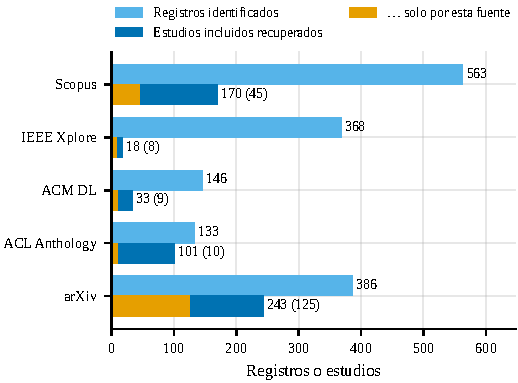
\includegraphics[width=\columnwidth,height=0.85\textheight,keepaspectratio]{busqueda_fuentes}
\caption{Registros identificados por fuente y estudios incluidos (brazo de bases) recuperados por cada fuente; entre paréntesis, los recuperados solo por esa fuente. Un estudio recuperado por varias fuentes cuenta en cada una; a cada registro conservado se le suman las fuentes de las versiones eliminadas antes del cribado.}
\label{fig:busqueda_fuentes}
\end{figure}


El \fechaBusqueda{} se consultaron \nBases{} fuentes: Scopus (\nBaseScopus{} registros), IEEE Xplore (\nBaseIEEE{}), ACM Digital Library (\nBaseACM{}), ACL Anthology (\nBaseACL{}) y arXiv (\nBaseArxiv{}), con un total de \nIdentificados{} registros. La \cref{fig:busqueda_fuentes} muestra, para cada fuente, los registros identificados y los estudios incluidos que recuperó, incluidos los que solo ella recuperó. Todas las cadenas siguen la misma estructura, que combina el bloque de la tarea con el bloque de multiturno o el de los pilares de vinculación y autocorrección. Las cadenas exactas, los campos y los filtros de cada fuente se incluyen en el \cref{app:busqueda}, conforme a PRISMA-S. Las cadenas estaban en inglés, de modo que las publicaciones en español pueden haberse omitido.

La captura difirió según la fuente. Scopus e IEEE Xplore se consultaron en sus interfaces web y se exportaron los resultados. ACM Digital Library no ofrece exportación a cuentas no premium, de modo que se guardaron las páginas de resultados en HTML sin editar y se extrajeron el DOI y el título de cada ítem; los demás metadatos se completaron por DOI desde OpenAlex y Crossref (enmienda A2). Para ACL Anthology se aplicó un \en{script} sobre el volcado oficial. Para arXiv se consultó la API con el bloque de la tarea y se filtró localmente por categoría de informática y por la cadena completa. Los registros se combinaron y deduplicaron con la herramienta de cribado (por DOI, y por título normalizado y año). Antes del cribado se eliminaron \nDupVersiones{} registros que eran versiones del mismo estudio, \nDupDOI{} duplicados por DOI erróneo y \nDupHerramienta{} detectados automáticamente por DOI o por título y año.

La sensibilidad de la búsqueda se midió con un conjunto de referencia, usado solo para esta medición (enmienda A1). La búsqueda recuperó \nRefMTHallados{} de \nRefMT{} estudios multiturno del conjunto (límite inferior de Wilson de \refMTICinf~\%) y \nRefUTHallados{} de \nRefUT{} estudios de un turno (IC 95~\% de Wilson, \sensUTInf--\sensUTSup~\%). Como la elegibilidad del conjunto la determinó la IA, el conjunto es circular y el límite inferior multiturno es una cota optimista, no una sensibilidad independiente. No se dispuso de un conjunto de referencia independiente, y no se consultaron DBLP ni Web of Science.

Los informes no recuperados se clasifican por una «señal» asignada a partir del título y el resumen: señal multiturno si contienen palabras clave de multiturno y señal de un turno en caso contrario. La señal no equivale a la elegibilidad, que solo se juzga con el texto completo (\cref{sec:met-sintesis}).

La búsqueda se complementó con \en{snowballing} hacia atrás y hacia adelante~\cite{Wohlin2014Snowballing}, sin iterar, desde \nBolaSemillas{} estudios semilla del Nivel 2. Se usó OpenAlex~\cite{Priem2022OpenAlex}, que aportó \nBolaCandOA{} candidatos. Para \nBolaSemillasSS{} semillas sin referencias en OpenAlex se recurrió a Semantic Scholar~\cite{Kinney2023SemanticScholar}, que dispuso de referencias para \nBolaSemillasSSrefs{} de ellas y aportó \nBolaCandSS{} candidatos. Los candidatos se filtraron con el bloque de la tarea sobre título y resumen y siguieron el mismo cribado en un espacio separado (enmienda A5b).

\subsection{Proceso de selección}
\label{sec:met-seleccion}
% PRISMA ítem 8 (proceso de selección; uso de herramientas de automatización)

% Generado por analysis/src/tablas/tablas.py — no editar a mano.
\begin{table*}[!tbp]
\centering
\caption{Uso de modelos de IA y acuerdo entre revisores por fase. En el cribado, $n$ son registros o informes y el acuerdo es sobre avanzar o excluir; en la extracción y la calidad, $n$ son estudios y el acuerdo es por campo o ítem. Verificación de la autora sin cambios: valores concordantes del Nivel 2, 182/182; filas del Nivel 1, 32/32; ítems de validez cerca del umbral, 95/95. \textsuperscript{a}Parte del Nivel 1 la revisó Codex con el mismo modelo para A y B (enmienda A5).}
\label{tab:ia}
\footnotesize
\begin{tabular}{@{}l r l l r r@{}}
\toprule
Fase & $n$ & Revisores A / B & Desempate & Acuerdo (\%) & $\kappa$ (PABAK) \\
\midrule
Cribado T/R (bases) & 1041 & Sonnet / Sonnet & Opus & \num{96.9} & \num{0.94} (\num{0.94}) \\
Texto completo (bases) & 431 & Sonnet / Sonnet\textsuperscript{a} & Opus & \num{97.0} & \num{0.92} (\num{0.94}) \\
Cribado T/R (bola de nieve) & 292 & Sonnet / Sonnet & Opus & \num{94.2} & \num{0.84} (\num{0.88}) \\
Texto completo (bola de nieve) & 58 & Sonnet / Sonnet & Opus & \num{93.1} & \num{0.84} (\num{0.86}) \\
Extracción, Nivel 1 & 317 & Sonnet / Sonnet & Codex & \num{86.9} & --- \\
Extracción, Nivel 2 & 78 & Sonnet / Codex & Sonnet & \num{73.6} & --- \\
Calidad, Nivel 2 & 78 & Sonnet / Codex & Sonnet & \num{75.6} & --- \\
\bottomrule
\end{tabular}
\end{table*}


El cribado se realizó con sr-screener, de la suite Academic Research Skills~\cite{ARS2026}. Cada registro lo evaluaron de forma independiente y cegada los revisores A y B (Claude Sonnet, con perfiles de experto distintos), que solo leían el archivo asignado y aplicaban los criterios del protocolo traducidos al inglés. Un tercer revisor (Claude Opus) resolvió los desacuerdos entre avanzar y excluir. Como A y B comparten familia de modelo, no se consideran revisores independientes en el sentido de Kitchenham; su acuerdo es solo un diagnóstico (\cref{tab:ia}), con $\kappa$ de Cohen~\cite{Cohen1960Coefficient} y PABAK~\cite{Byrt1993Bias}. Los identificadores exactos de los modelos, los ajustes de ejecución y una plantilla de \en{prompt} por etapa figuran en el \cref{app:ia}; las decisiones de cada registro, con su motivo, se archivan en el repositorio del proyecto.

La verificación humana siguió el diseño de la enmienda A3. La autora etiquetó a ciegas, antes de conocer la decisión de la IA, una muestra de \nPiloto{} registros que sirvió de piloto y de validación. La autora avanzó \nPilotoAvanzaAutora{} de ellos, la IA omitió \nPilotoOmitidosIA{} y $\kappa$ fue \pilotoKappa{}. La autora revisó además todos los casos no evidentes en que la IA podía excluir un estudio: \nConflictosTR{} conflictos entre revisores y las exclusiones que la recomprobación proponía avanzar, con lo que decidió \nAutoraTR{} registros en título y resumen. Las exclusiones conjuntas de A y B no pasan por el desempate. De las \nConjuntas{} exclusiones conjuntas, \nNoReleidas{} no se releyeron; un segundo lector cegado (Claude Opus) releyó \nQC{} de ellas (\nQCCercanos{} cercanas a los criterios por palabras clave y \nQCAleatorios{} aleatorias). % NOTA: \nQC (401) + \nNoReleidas (80) = 481, no \nConjuntas (477); conciliar con la autora la diferencia de 4 registros antes de publicar.
Esa lectura avanzó \nQCAvanzados{} registros, de los que se incluyeron finalmente \nQCIncluidos{}. En el estrato aleatorio se incluyeron finalmente \nRescAleat{} de \nAleatRel{} (\tasaRescate~\%, IC 95~\% de \tasaRescateInf{} a \tasaRescateSup~\%), lo que, extrapolado a las exclusiones no releídas, equivale a \omisEsp{} estudios omitidos esperados (IC 95~\% de \omisEspInf{} a \omisEspSup{}).
% fuente: revision_4f.json (A5_omisiones)

En texto completo, los revisores A y B fueron Claude Sonnet (enmienda A5a). Los informes sin decisión previa se cribaron con un extracto (páginas iniciales y sección experimental), calibrado frente al texto completo: Claude coincidió en \nCalibClaude{} de \nCalibN{} informes y Codex en \nCalibCodex{} de \nCalibN{}, en la decisión de incluir o no. Una parte del Nivel 1 la revisó GPT Codex, con el mismo modelo para A y B de cada informe; Claude auditó \nAuditN{} de \nAuditPool{} inclusiones de Codex y confirmó \nAuditOK{}. Opus realizó una segunda lectura de los \nQCTCdudosos{} informes dudosos y de las \nQCTCmt{} exclusiones conjuntas por el criterio E6 con señal multiturno. Se registraron \nConflictosTC{} conflictos, de los que el adjudicador resolvió \nAdjTC{}, y la autora decidió \nAutoraTC{} informes.

No se contactó a los autores de los informes no recuperados (enmienda A4). La recuperación usó rutas abiertas automáticas y la búsqueda manual de la autora; los informes no obtenidos se reportan en el diagrama PRISMA, se describen por escenario y se incorporan a un análisis de sensibilidad de D4.

\subsection{Extracción de datos}
\label{sec:met-extraccion}
% PRISMA ítems 9, 10a y 10b

El formulario de extracción, con vocabularios controlados y la ubicación de cada valor, figura en el \cref{app:formulario}. La extracción tiene dos niveles (D7). El Nivel 1 cubre todos los estudios, se extrae de las páginas iniciales de cada informe e incluye la caracterización, el escenario, los pilares centrales y los códigos de técnica de PI3 y PI4. El Nivel 2 aplica el formulario completo a los estudios multiturno (PI1–PI5, resultados por \en{benchmark}, métrica y turno, y contrastes dentro del estudio). Las ejecuciones de extracción de la \cref{tab:ia} (\nExtrNivelUno{} del Nivel 1 y \nExtrNivelDos{} del Nivel 2) suman más que los \nEstudios{} estudios porque \nReclasificados{} estudios reclasificados se extrajeron en ambos niveles; la división final es de \nUnTurno{} estudios de un turno y \nMultiturno{} multiturno.

La extracción fue doble y estuvo a cargo de la IA, con comparación automática y reglas de resolución preespecificadas (enmienda A5c). En el Nivel 1, los revisores A y B fueron Claude Sonnet y el desempate lo hizo Codex. En el Nivel 2, A fue Claude Sonnet, B fue Codex y el desempate lo hizo Sonnet sobre las páginas citadas. El acuerdo entre A y B en el Nivel 2 antes de la resolución, por campo, fue de \acuerdoCampoPilaresCentrales{} en los pilares centrales, \acuerdoCampoTecnicaContexto{} en la técnica de restauración del contexto, \acuerdoCampoRepresentacion{} en la representación del estado, \acuerdoCampoInferenciaJoins{} en la inferencia de \en{joins}, \acuerdoCampoMecanismo{} en el mecanismo de PI4 y \acuerdoCampoHistorial{} en el historial de la evaluación. La puntuación de calidad se obtuvo en las mismas llamadas. La autora revisó las discrepancias no resueltas, una muestra aleatoria de los valores concordantes del Nivel 2 (\verifC{} confirmados sin cambios), una muestra de filas del Nivel 1 (\verifD{}) y los ítems de validez cercanos al umbral (\verifB{}). Además, extrajo y puntuó a ciegas \nMuestraCiega{} estudios del Nivel 2, antes de ver la propuesta de la IA. Se añadió la variable \texttt{foro\_nivel} (enmienda A5d), con el nivel CORE para congresos y el cuartil SJR para revistas, solo para análisis de sensibilidad y no como criterio de elegibilidad.
% fuente: revision_4f.json (A5_acuerdo_campo_nivel2)

El desenlace primario es EX. Los secundarios son EM/ESM y TS y, en multiturno, QM/IM. También se extrajeron la degradación por turno y los contrastes dentro del estudio, definidos como un componente activado frente a desactivado con el mismo modelo base, además de las variables de la \cref{sec:met-picoc}.

\subsection{Evaluación de la calidad}
\label{sec:met-calidad}
% PRISMA ítem 11

La calidad de los estudios del Nivel 2 se evaluó con una lista de \nItemsCalidad{} ítems al estilo de Kitchenham, adaptada a Text-to-SQL; no se usaron RoB~2 ni ROBINS-I, diseñadas para estudios de intervenciones en salud. Cada ítem se puntúa como completo, parcial o ausente. Solo los \nItemsValidez{} ítems de validez (CQ2 y CQ4–CQ7) determinan la puntuación de validez; un estudio entra a la síntesis en profundidad si alcanza al menos \umbralValidez{}~\%. El umbral del \umbralValidez{}~\% se registró en el protocolo y excluye pocos estudios, por lo que la lectura con todos los estudios (la sensibilidad ya realizada) es igualmente informativa. Los estudios de un turno (Nivel 1) no se evaluaron en calidad, de modo que los contrastes con ellos carecen de evaluación. Los ítems de reporte y apertura (CQ1, CQ3, CQ8–CQ10) se reportan por ítem, mediante un perfil tipo semáforo, y no se suman. El ítem CQ10 considera los indicios de prácticas depredadoras según \emph{Think. Check. Submit.}~\cite{TCS2026}. La autora y la IA calibraron la lista con \nCalibCalidad{} estudios. La puntuación la propuso la IA con doble lectura (\cref{sec:met-extraccion}), con verificación por muestreo.

\subsection{Síntesis}
\label{sec:met-sintesis}
% PRISMA ítems 12, 13a--13f, 14 y 15

La síntesis es narrativa y estructurada según SWiM~\cite{Campbell2020SWiM}, sin metaanálisis. Los grupos son los niveles (D7) y las clases de componente de PI1–PI4. Solo se comparan valores dentro de una misma configuración (\en{benchmark}, versión, partición, métrica, tipo de historial y conocimiento externo). La evidencia principal sobre el efecto de un componente son los contrastes dentro del estudio, resumidos con mediana, rango y dirección. La diferencia frente a la línea base de referencia, con el mismo modelo base, es evidencia secundaria. Las comparaciones entre estudios son descriptivas y no prueban superioridad. Las categorías abiertas se consolidaron de forma inductiva, y los valores no reportados se mantienen como tales.

El indicador D4 es la proporción de estudios multiturno entre los que abordan la vinculación de esquemas o la autocorrección como contribución central, con intervalo de Wilson~\cite{Wilson1927Probable}. Según la regla preespecificada, se concluye que el escenario es considerablemente menos investigado solo si el límite superior es de a lo sumo \umbralDcuatro{}~\%; si el intervalo contiene ese valor, el resultado es no concluyente. D4 es una proporción descriptiva dentro del marco de elegibilidad, no una afirmación sobre todo el campo. El umbral del \umbralDcuatro{}~\% es una referencia descriptiva fijada en el protocolo. El intervalo de Wilson cubre solo el error muestral, no el de clasificación ni el de selección; por ello se reporta además el acuerdo en el campo que define D4 (pilares PI3/PI4 centrales, Nivel 1). La tendencia anual de 2019 a 2025 se evalúa con la prueba de Cochran--Armitage~\cite{Cochran1954Methods,Armitage1955Tests} por permutación (\replicasTendencia{} réplicas); 2026 se reporta aparte por ser un año parcial, y como sensibilidad se repite la prueba incluyéndolo, sin sustituir a la prueba registrada. Las curvas y pendientes de degradación se estratifican por el tipo de historial usado en la evaluación (GOLD, PREDICHO o SOLO\_PREGUNTAS) y nunca se agrupan, y solo el estrato PREDICHO se interpreta como propagación de errores.

Las sensibilidades excluyen los preprints, reincorporan los estudios bajo el umbral, usan la versión laxa de D4, restringen D4 a las búsquedas en bases, consideran los foros de primer nivel e incorporan los informes no recuperados, mediante una cota extrema (todos cuentan en el denominador y los de señal multiturno también en el numerador) y una estimación probabilística que aplica las tasas observadas entre los informes recuperados. El sesgo de notificación se considera en los contrastes dentro del estudio, la contaminación de \en{benchmarks}, el desfase de líneas base y la recuperación diferencial por escenario. En los contrastes se cuentan además los nulos con un umbral de $|\Delta| <$ \umbralNulo{}~pp, y se añade una lectura que rebaja un nivel la confianza por sesgo de notificación; esta lectura penalizada es una sensibilidad añadida y la regla registrada no cambia. La confianza de cada hallazgo, inspirada en GRADE-CERQual~\cite{Lewin2018CERQual}, combina las limitaciones metodológicas, la coherencia, la suficiencia y la pertinencia con reglas propias, que no equivalen a una aplicación validada de CERQual. Por último, un análisis bibliométrico exploratorio (enmienda A6) describe la comunidad del foro y la red de citas, y se etiqueta como tal.
